\section{Additional figures}

\subsection{$\rm{KE_{T}}$ scaling}
\label{Subsubsection:KETscaling}

One suggestion to further study the scaling properties of flow coefficients was to extend the scaling to lower \pT~values by studying the transverse kinetic energy dependence of anisotropic flow harmonics. Transverse kinetic energy is defined as ${\rm KE}_{\rm{T}} = m_{\rm{T}} - m_{\rm{0}}$, where $m_{\rm{T}}= \sqrt{m_{0}^2 + p_{\rm{T}}^2}$ is the transverse mass. Figures \ref{v422_KET}, \ref{v523_KET}, \ref{v633_KET} and \ref{v6222_KET} present ${\rm KE}_{\rm{T}}$ scaling for $v_{4,22}$, $v_{5,32}$, $v_{6,33}$ and $v_{6,222}$ respectively, for \pion, \kaon, \proton, \Ks, \lambdas~and $\phi$-meson grouped in different centrality intervals.

\begin{figure}[htb]
\begin{center}
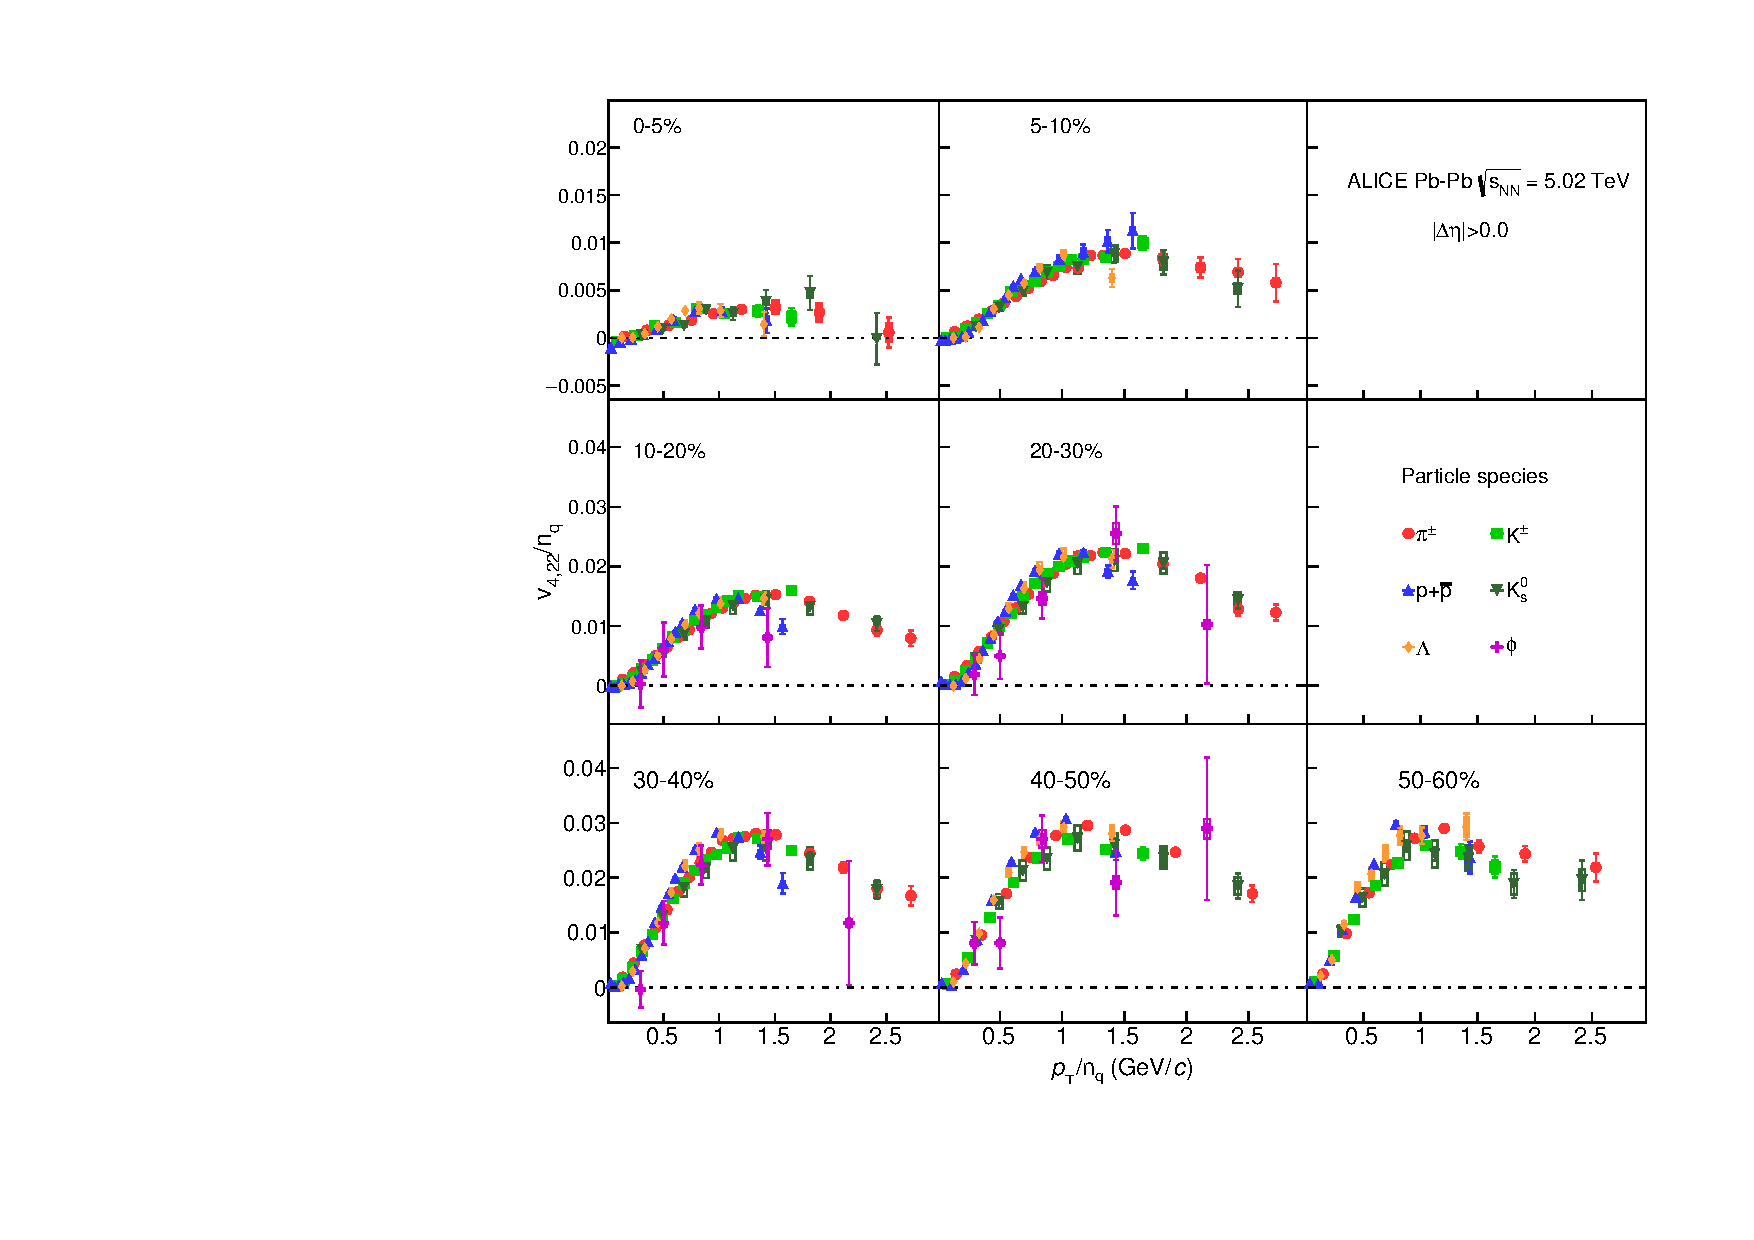
\includegraphics[scale=0.82]{figures/scaling/All_v422_gap00_KET_3by3.pdf}

\end{center}
\caption{The $(m_{\rm{T}} - m_{0})/n_{q}$-dependence of $v_{4,22}/n_{q}$ for different particle species grouped into different centrality intervals of Pb--Pb collisions \sNN. Statistical and systematic uncertainties are shown as bars and boxes, respectively. It is seen that the $\rm KE_{T}$ scaling holds for $v_{4,22}$ at an approximate level.}
\label{v422_KET}
\end{figure}

\begin{figure}[htb]
\begin{center}
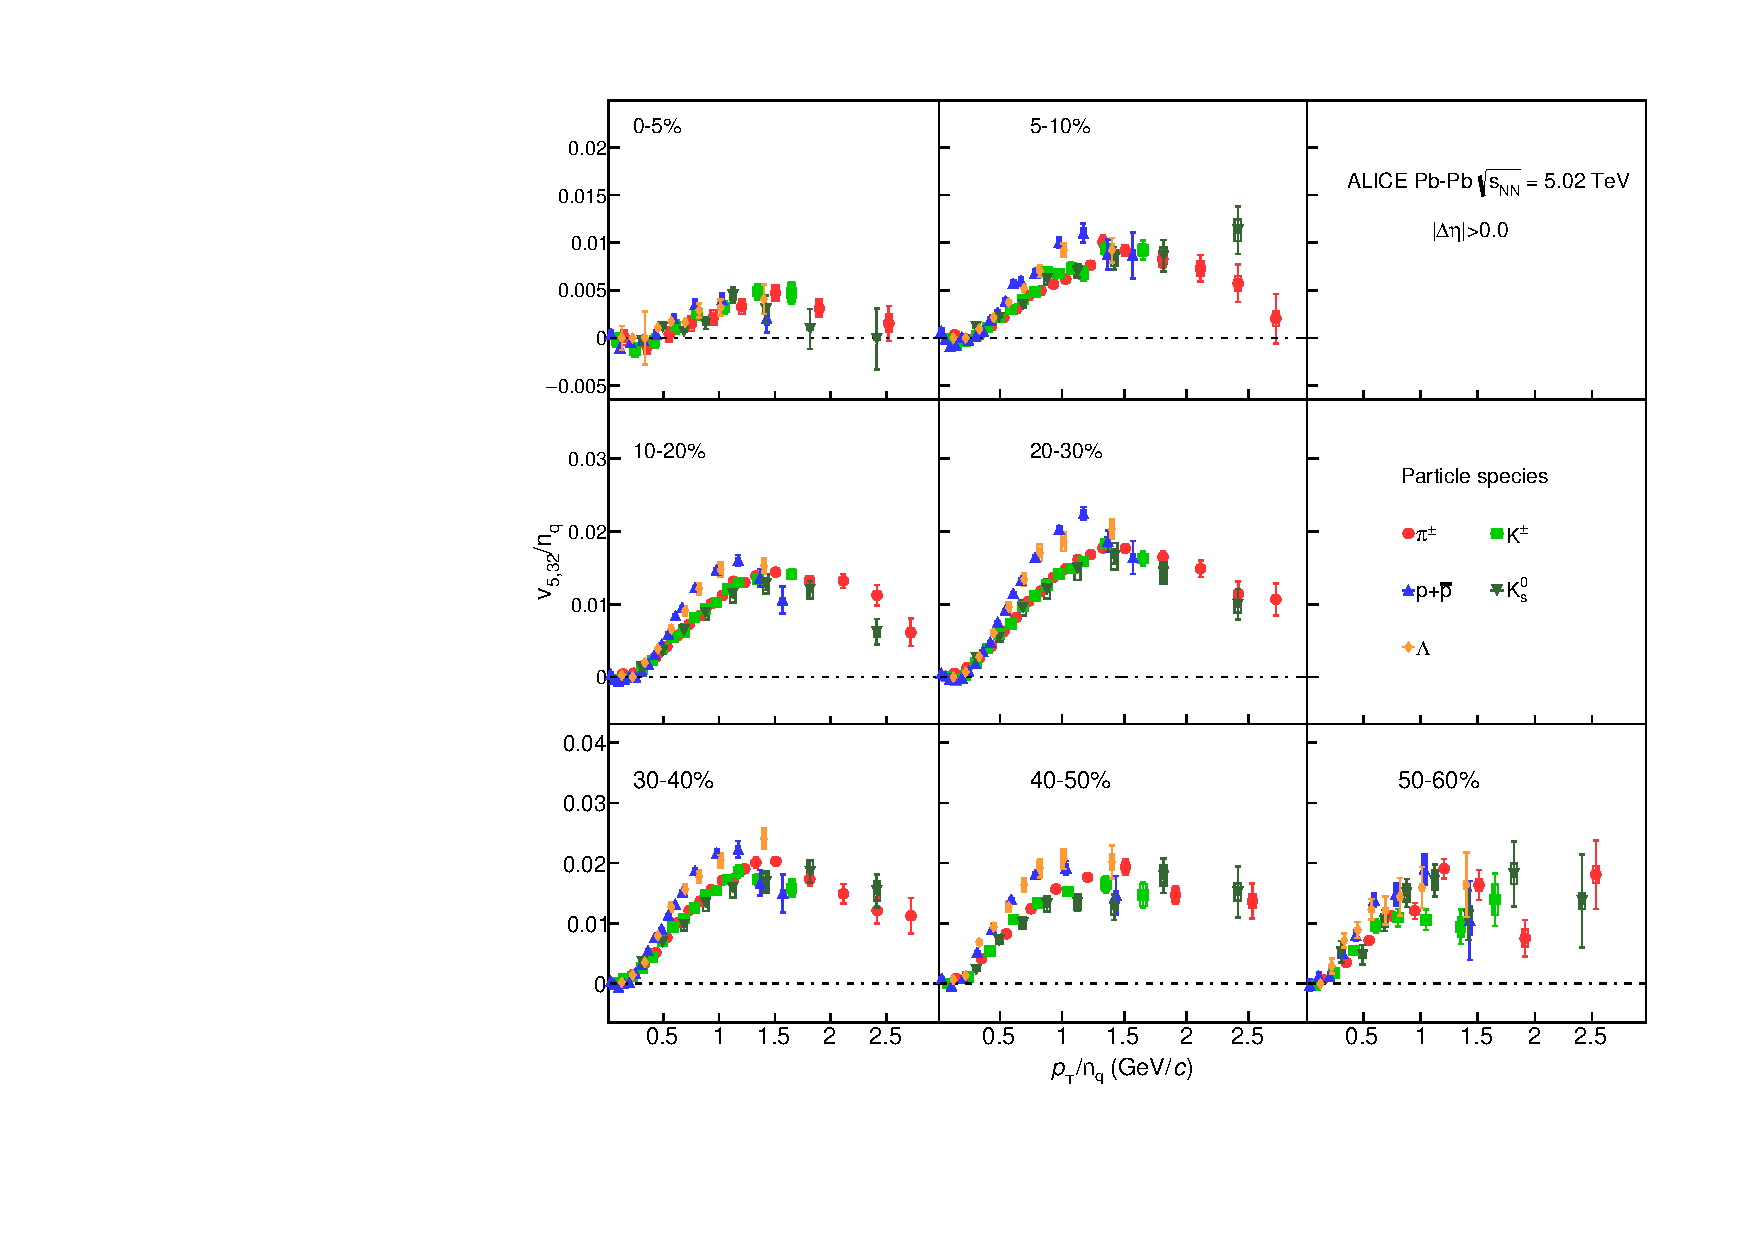
\includegraphics[scale=0.82]{figures/scaling/All_v523_gap00_KET_3by3.pdf}
\end{center}
\caption{The $(m_{\rm{T}} - m_{0})/n_{q}$-dependence of $v_{5,32}/n_{q}$ for different particle species grouped into different centrality intervals of Pb--Pb collisions \sNN. Statistical and systematic uncertainties are shown as bars and boxes, respectively. It is seen that the $\rm KE_{T}$ scaling holds for $v_{5,32}$ at an approximate level.}
\label{v523_KET}
\end{figure}

\begin{figure}[htb]
\begin{center}
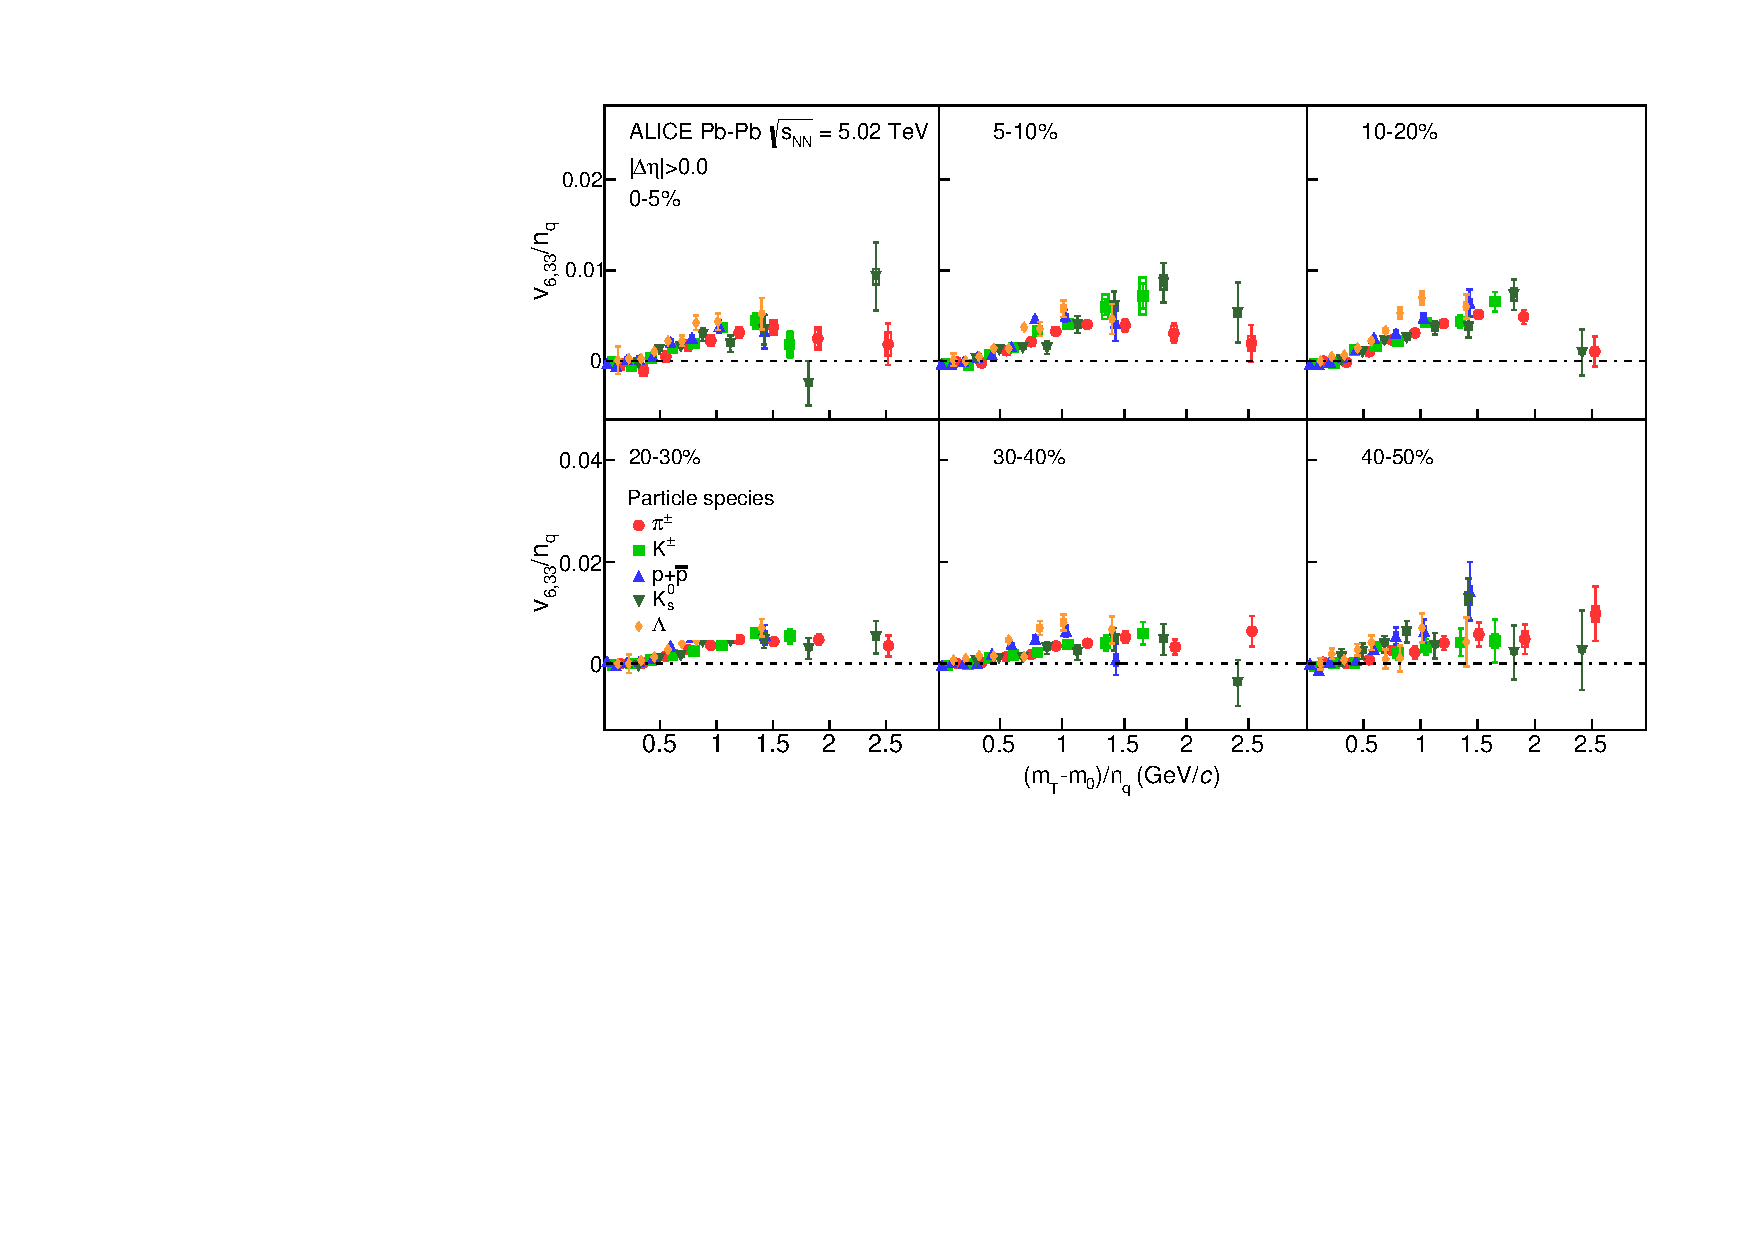
\includegraphics[scale=0.82]{figures/scaling/All_v633_gap00_KET_3by2.pdf}
\end{center}
\caption{The $(m_{\rm{T}} - m_{0})/n_{q}$-dependence of $v_{6,33}/n_{q}$ for different particle species grouped into different centrality intervals of Pb--Pb collisions \sNN. Statistical and systematic uncertainties are shown as bars and boxes, respectively. It is seen that the $\rm KE_{T}$ scaling holds for $v_{6,33}$ at an approximate level.}
\label{v633_KET}
\end{figure}

\begin{figure}[htb]
\begin{center}
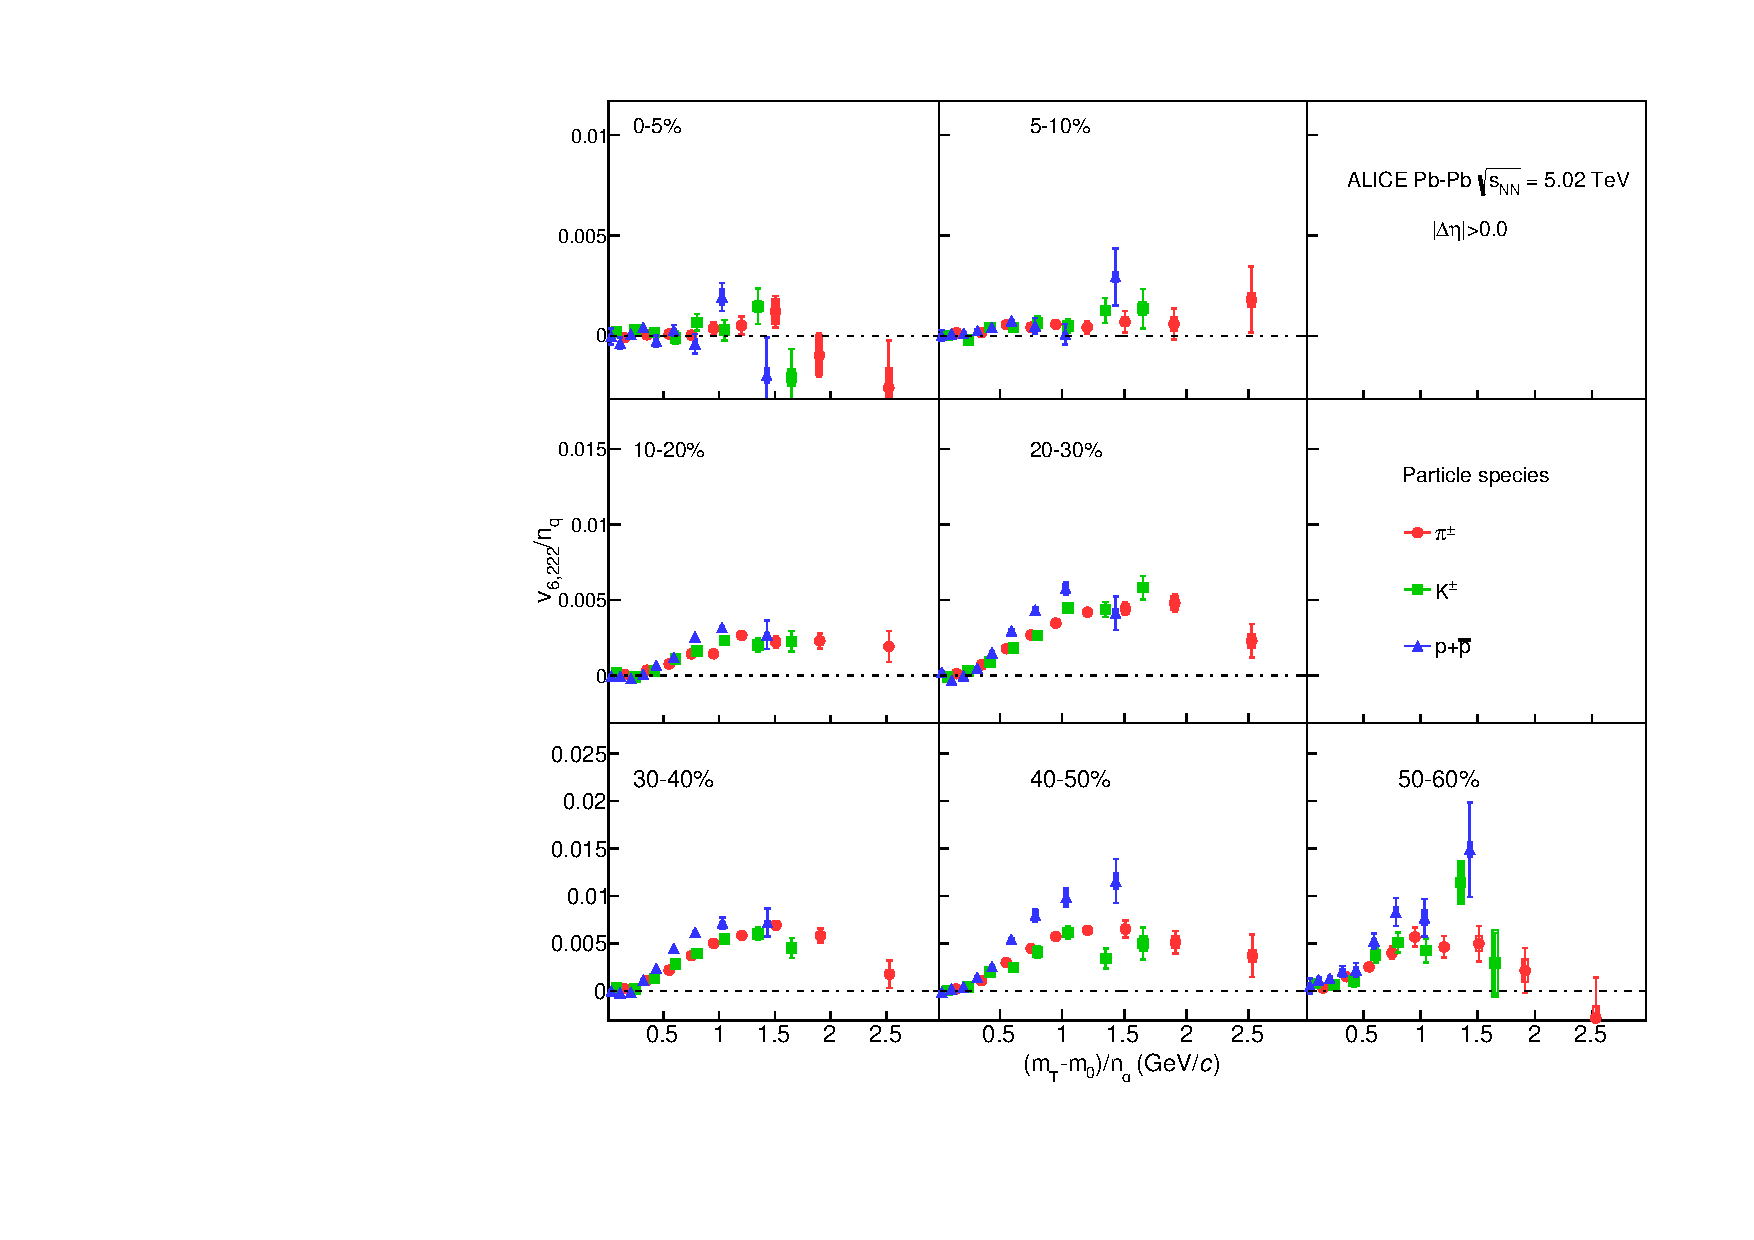
\includegraphics[scale=0.82]{figures/scaling/All_v6222_gap00_KET_3by3.pdf}
\end{center}
\caption{The $(m_{\rm{T}} - m_{0})/n_{q}$-dependence of $v_{6,222}/n_{q}$ for different particle species grouped into different centrality intervals of Pb--Pb collisions \sNN. Statistical and systematic uncertainties are shown as bars and boxes, respectively. It is seen that the $\rm KE_{T}$ scaling holds for $v_{6,222}$ at an approximate level.}
\label{v6222_KET}
\end{figure}